\documentclass{article}        	
\usepackage{amsfonts, amssymb, amsmath, graphicx, pgfplots, tikz, fancyhdr}
\pgfplotsset{compat=1.17}
\usepackage[a4paper, margin=0.8in]{geometry}

\fancypagestyle{main}{
    \fancyhf{} % Limpia encabezados y pies de página
    \fancyhead[C]{Juan Ignacio Elosegui} % Encabezado centrado con tu nombre
    \fancyfoot[R]{\thepage} % Número de página alineado a la derecha en el pie
    \renewcommand{\headrulewidth}{0.4pt} % Línea bajo el encabezado
    \renewcommand{\footrulewidth}{0pt}   % Sin línea en el pie de página
}

\pagestyle{main}

\begin{document}
    \section*{Ejercicio Carrera}
        Se tiene una clase Carrera que representa una carrera de atletismo. La carrera tiene un conjunto de participantes, cada uno con un identificador único y un nombre único.
        
        Además, se registra el tiempo y la posición de llegada de cada participante que finaliza la carrera. \\
        A continuación se detalla la estructura de representación elegida. Escribir en español y en lenguaje formal el invariante de representación de la misma.  
        \begin{center}
            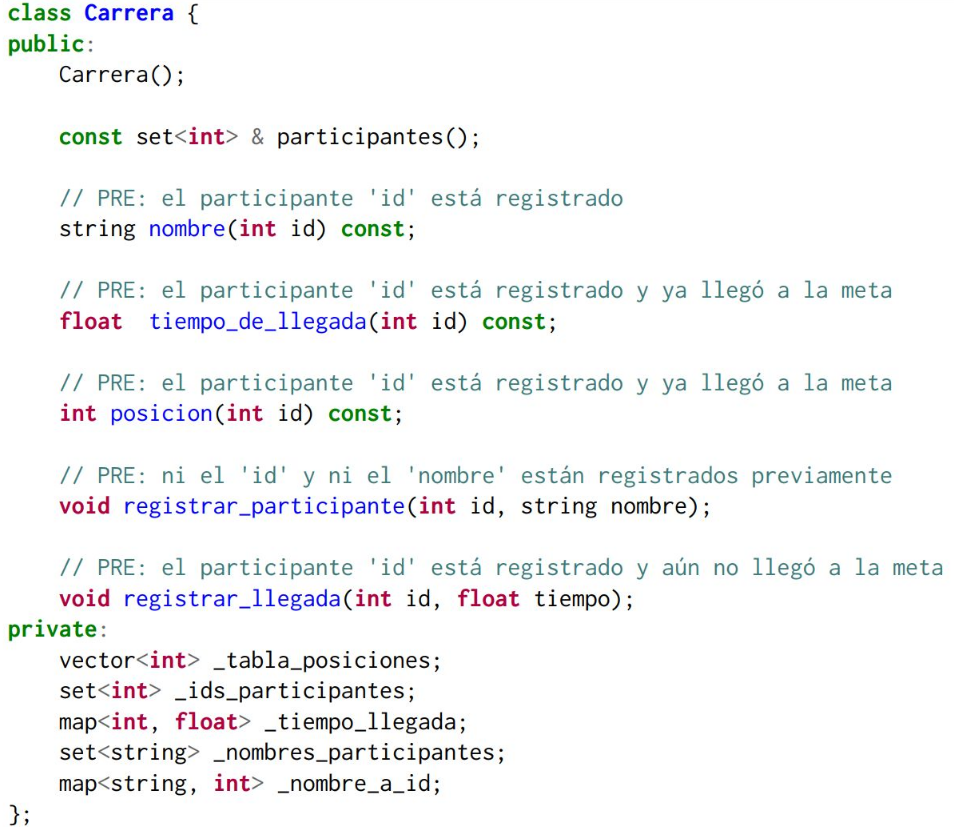
\includegraphics[width=0.8 \linewidth]{img/carrera.png}
        \end{center}
    \newpage
        \subsection*{Propiedades individuales}
            \subsubsection*{En español:}
                \texttt{\_tabla\_posiciones} tiene como mínimo un elemento. Para que sea una carrera, tiene que haber alguien corriendo, o, si se quiere, dos personas como mínimo. Esas personas estarán representadas con un ID. \\
                \\
                \texttt{\_ids\_participantes} es un conjunto que no tiene elementos repetidos (porque es un conjunto) y puede ser cualquier cosa el número del ID, depende de qué método de identificación se use. Los IDs son los participantes de la carrera. \\
                \\
                \texttt{\_tiempo\_llegada} tendrá como claves los IDs de los participantes, y como valor tendrá el tiempo que tardaron en correr (si no terminó, se pone como tiempo cero). Como es de esperar, el tiempo de llegada es un valor positivo y distinto de cero. No tiene elementos repetidos. No hay elementos repetidos. \\
                \\
                \texttt{\_nombres\_participantes} no tiene elementos repetidos, y contiene los nombres de los participantes. Estos nombres están representados como strings, y no pueden ser vacíos. \\
                \\
                \texttt{\_nombre\_a\_id} tiene los nombres en strings asociados a IDs. Los strings no pueden ser vacíos.
            \subsubsection*{En lógica formal:}
                \texttt{\_tabla\_posiciones}: \( |e.\texttt{\_tabla\_posiciones}| \geq 2 \). \\
                Asumiendo que el método de identificación es arbitrario (no se pide nada específico en cuanto a esto) y deben correr como mínimo dos personas. \\
                \\
                Skippeo esto porque, como es un conjunto, claramente no va a tener elementos repetidos. \\
                \\
                \texttt{\_tiempo\_llegada}: \( (\forall \texttt{id:int}) (\texttt{id} \in claves(e.\texttt{\_tiempo\_llegada}) \Rightarrow e.\texttt{\_tiempo\_llegada}[\texttt{id}] \geq 0) \) \\
                \\
                \texttt{\_nombres\_participantes}: \( (\forall \texttt{s:string} \in e.\texttt{\_nombres\_participantes}) \Rightarrow (|\texttt{s}| \geq 1) \) \\
                \\
                \texttt{\_nombre\_a\_id}: \( (\forall \texttt{s:string} \in claves(e.\texttt{\_nombre\_a\_id})) \Rightarrow |e.\texttt{\_nombre\_a\_id[s]}| \geq 1 \)
        \subsection*{Relaciones}
            \subsubsection*{En español:}
                En cuanto a tamaños, \texttt{\_tabla\_posiciones} tiene el mismo tamaño que el cardinal de \texttt{\_ids\_participantes}, que la cantidad de claves en \texttt{\_tiempo\_llegada} y \texttt{\_nombre\_a\_id}, y que el cardinal de \texttt{\_nombres\_participantes}. \\
                \\
                Los elementos de \texttt{\_ids\_participantes} son los mismos valores asociados en \texttt{\_nombre\_a\_id}, las mismas claves que en \texttt{\_tiempo\_llegada} y deben estar presentes en \texttt{\_tabla\_posiciones}. \\
                \\
                Los elementos de \texttt{\_nombres\_participantes} son también las claves en \texttt{\_nombre\_a\_id}.
            \subsubsection*{En lógica formal:}
                \textit{Alta paja de hacerlo. Por hoy, me fundí.}
\end{document}